\documentclass[letterpaper,twocolumn,10pt]{article}
\usepackage{usenix-2020-09}

% to be able to draw some self-contained figs
\usepackage{tikz}
\usepackage{amsmath}
\hypersetup{hidelinks}

%-------------------------------------------------------------------------------
\begin{document}
%-------------------------------------------------------------------------------

%don't want date printed
\date{}

% make title bold and 14 pt font (Latex default is non-bold, 16 pt)
\title{\Large \bf Lab 2: Fuzzing LibPNG}

%for single author (just remove % characters)
\author{
{\rm Kenji Rohner}\\
ETHZ
\and
{\rm Botond Kovacs}\\
EPFL
\and
{\rm Cesar Ernesto Illanes Argote}\\
EPFL
\and
{\rm Alexandre Margery}\\
EPFL
% copy the following lines to add more authors
% \and
% {\rm Name}\\
%Name Institution
} % end author

\maketitle

\vspace{-1.5em}
\begin{center}
{\scriptsize Repository link: \href{https://github.com/ImYuushi/SoftSec-Lab-2-Group33}{\texttt{github.com/ImYuushi/SoftSec-Lab-2-Group33}}}
\end{center}
\vspace{-1em}

%Q1
%-------------------------------------------------------------------------------
\section{Harness Design}

The first decision to make is what library to fuzz. Ultimately, we have decided on libPNG. As the reference library for handling PNGs, having been active for over 30 years, it is a prime target for this exercise, with many older versions to fuzz and security fixes to recreate. Specifically, we chose to target version 1.2.56, as targeting an older version increases the chances of finding a bug.

Fuzzing a library is a very different endeavour from fuzzing a regular program. Unlike a regular program, a library does not have a well-defined "start" to its code. As such, the choice of entry point can make a huge difference to the results and effectiveness of the fuzzing. For this we used three different entry points. By using preprocessor Macros, we compiled three different Binaries. These Binaries test the progressive reader: png\_set\_progressive\_read\_fn(), the png\_read\_image() function and some transform functions. For the first two, the read functions, the rational was the same: they are the most important part of the library, since every call of libpng most likely requires a PNG to be read and thus one of the read functions to be called. We also wanted to see if reading those images and messing with the inputs could cause a crash when we not just read the images but we also used transforms on them.

%Q2
%-------------------------------------------------------------------------------

\section{Instrumentation and Sanitizers}

The next step was to set up the instrumentation and sanitizers. We set up three version of libpng: An AFL++ instrumented built without sanitizers, an AFL++ instrumented build with AddressSanitizer, and an uninstrumented build that will be used later for QEMU mode. The AFL compilations are done with afl-clang-fast to allow AFL to receive coverage feedback, and do coverage-guided fuzzing.  In terms of Optimization and Debug flags, we applied -O1, enabling moderate optimization at fairly low cost to the fuzzing process. Higher optimization levels would be possible, and improve the overall fuzzing speed, but would significantly reduce observability. We also added the -g flag, adding helpful debug symbols such as stack-traces and GDB triage, which allows easier crash debugging. We also applied --disable-shared, to make sure AFL reliably loads the instrumented version; without it it is possible that a non-instrumented, separately-installed version would be used.

For sanitizers, we added ASan which allows detection of heap overflows, stack overflows, use-after-free bugs, invalid reads/writes, and other memory corruption issues, overall significantly improving bug detection quality during fuzzing. However, it comes at the cost of significant slowdowns due to shadow memory checks, allocator instrumentation, and additional bookkeeping. While running the campaign without ASan would improve fuzzing throughput, it would also mean that we could not detect many memory safety violations, as they would fail to crash reliably, which is contrary to the purpose of the fuzzing campaign.
For patches, we applied libpng-nocrc.patch, a patch designed to loosen the CRC/checksum validation in libpng. This is meant to improve fuzzing performance by allowing mutated inputs to get further into the parsing pipeline. Without it, many inputs would be stopped very early due to incorrect checksums.

Finally, for environment variables, we set AFL\_SKIP\_CPUFREQ and AFL\_I\_DONT\_CARE\_ABOUT\_MISSING\_CRASHES to 1, as this improves AFL's ability to function inside a container, where its access to CPU measurements might not be reliable. We also enabled AFL\_AUTORESUME for faster and easier iteration during fuzzing.

%Q3
%-------------------------------------------------------------------------------

\section{Seed Corpus and Dictionary}
Another element that can greatly improve fuzzing performance is the presence of good, varied seeds, and a coherent dictionary. For seeds, we decided to create two "basic" seeds of simple, valid PNGs. Then, we have additionally added a grayscale PNG to reach some different execution paths, and a fully transparent PNG to create an interesting edge case. These ensure the fuzzing mutation starts from valid PNGs rather than random noise, allowing them to get much further into the execution path from the start. Looking at the queue entries in our results folder for the progressive fuzzing run, we can see that the vast majority of entries came from the grayscale seed (around 75), while a smaller portion have come from the transparent seed (around 20), The two "standard seeds" being responsible for very few entries overall. This is likely due to the fact that the grayscale PNG is handled differently from the usual RGB images, which allows that seed to trigger a large variety of special cases and extra branches specifically designed to handle grayscale images or transparent alpha channels. It is interesting to note that in the read\_png results queue, the standard PNGs contribute a much more significant fraction of the entries. This is likely due to the fact that as it has a more general decoding purpose, this entry point leads to less special treatment for the unusual PNGs, and more general approaches behind the scenes.

Additionally, we used a dictionary, which contains a variety of common PNG chunk identifiers and magic values. This can be a good tool to improve fuzzing performance by allowing the mutations to target specific sections of the file, ensuring less malformed files, and more valid PNGs that get deeper into the execution. This is especially useful for PNGs, which are very structured files where random mutations could destroy chunk names, lengths, or other important elements. From the AFL++ status screen we see that while it did attempt many usages of the dictionary, they didn't find much success, with the vast majority of new entries instead having been from the Havoc strategy. It is interesting to note that although we applied a patch to reduce checksum validation, deterministic mutation strategies such as bit flips, byte flips, arithmetic, and known ints still led to very few new paths. This is likely because PNG remains a highly structured format even without checksum enforcement. Mutations are very likely to corrupt chunk lengths, ordering, compression, or other necessary parsing elements. This also greatly damages the dictionary strategies: Unlike some file formats where keywords can appear meaningfully almost anywhere in the file, PNG expects its keywords in very specific spots: Adding "PLTE" somewhere in the middle of a PNG is unlikely to lead to a valid file libpng will recognize.

%Q4
%-------------------------------------------------------------------------------

\section{Campaign Analysis}

As shown in Figure~\ref{fig: statusInstru}, the stability is 100\%, corpus count is 252, map density is 7.05\% / 17.18\% and the number of cycles done is 24.

As for the edge curve shown in Figure~\ref{fig: edgeInstru}, there is rapid growth at the beginning, between t=0s and t=200s, the number of edges goes from 510 to 550, then there is a slower but consistent growth between t=200s and t=1350s where the number of edges increases from 550 to 570. There is then a sudden jump in a few seconds from 570 to 585 edges. From then on t=1380 until the end, there is a consistent slow growth. As such we do not seem to have reached saturation, although the rate of discovery has decreased, new edges are still being found until the end.

%Q5
%-------------------------------------------------------------------------------

\section{Crash Triage}

Unfortunately our testing with all three binaries, read\_image, progressive, and transforms did not yield any results. We then made another binary which contains a memory read\_error in the original harness, contained in a preprocessor macro. This binary is called fuzz\_fuzz\_induced\_bug. It has an OOB memory read. Running this with AFL clearly crashes and AFL catches it.

As for why no bugs were found: our approach was focused more on reading in the images in different ways. It is quite possible that this, in itself, is not a problem. Reading files that are malformed usually cause a problem down the line, when working on the picture, transforming it. While we have a binary that uses the transforms, they do not process them further and crashes would have already been found with fuzzing previously.

%Q6
%-------------------------------------------------------------------------------
\section{Attack Surface Analysis}

Similar to FFMPEG for videos, libpng is used widely in browsers and servers processing working pictures, since they are mostly in PNG format. By itself, a crash found by our program would probably not cause too much damage, but if we found memory corruptions, these might be able to be used in conjunction with other bugs on the server or in the browser.

Another possible use is in Embedded Systems. Since libpng is very lightweight and in C, it can easily be used in smaller devices with limited computing power. If our program found a crash in such a common function, then it might be possible to DoS these devices, since such small devices usually don't have a lot of redundancies and restarting crashed programs on devices like these is rather time-intensive. 

%Q7
%-------------------------------------------------------------------------------
\section{Binary-Only Fuzzing with QEMU mode}

We have also run a QEMU fuzzing campaign, in binary-only mode, without any sanitizers. As it can be seen in Figure~\ref{fig: 7.1} and Figure~\ref{fig: 7.2} of the appendix, this campaign actually had a significantly higher performance, in terms of average execution speed (2.72M in 30 mins vs 963k in 30), edges discovered ($\sim 1950$ vs $\sim 600$), and even corpus count (360 vs 250). This is a little surprising, as instrumented fuzzing is generally expected to be more performant than binary-only fuzzing, but a possible explanation here lies in the executions number; Instrumented fuzzing uses sanitizers, including ASan which can be anywhere from a 2x to a 5x slowdown. This would track with the ~3x reduction in executions which allows QEMU mode to move much faster through the fuzzing process. This is especially important for a fuzzing target such as libpng, dominated by early parser exits from invalid/malformed PNGs, which increases the importance of raw execution throughput compared to more precise instrumentation, especially for shorter fuzzing campaigns. The two campaigns were also run by different team members, so it is possible that hardware differences could have contributed to the performance gap, if the team member responsible for QEMU mode happens to have a more performant laptop.

%Q8
%-------------------------------------------------------------------------------

\section{Instrumentation Depth and Performance}

We can see that the map-density at the end of our instrumented run is 17.18\%. The reasons it does not reach most of the edges are varied, but the most important factor is the fact that a library as wide and mature as libpng will have many very specific feature paths, for handling a great number of niche PNGs, and niche ways to operate on them. Most of these will not have been reached by our fuzzing campaign simply due to their specificity, and the fact that 30 minutes is very short for a fuzzing campaign. 

In total we have 3475 possible instrumented edges, of which in progressive we have reached 603. 

When comparing execs speed we have the mode with no sanitizer at about 5600 execs per seconds and the other two at 134 executions per seconds. To explain why this happens one needs to understand what ASan does. It is basically a checker for memory errors. These kind of checks are very resource intensive, considering the whole memory has to be mapped among other things. This would explain the difference in execution speed by a magnitude.

\clearpage

\appendix
\begin{figure}
    \centering
    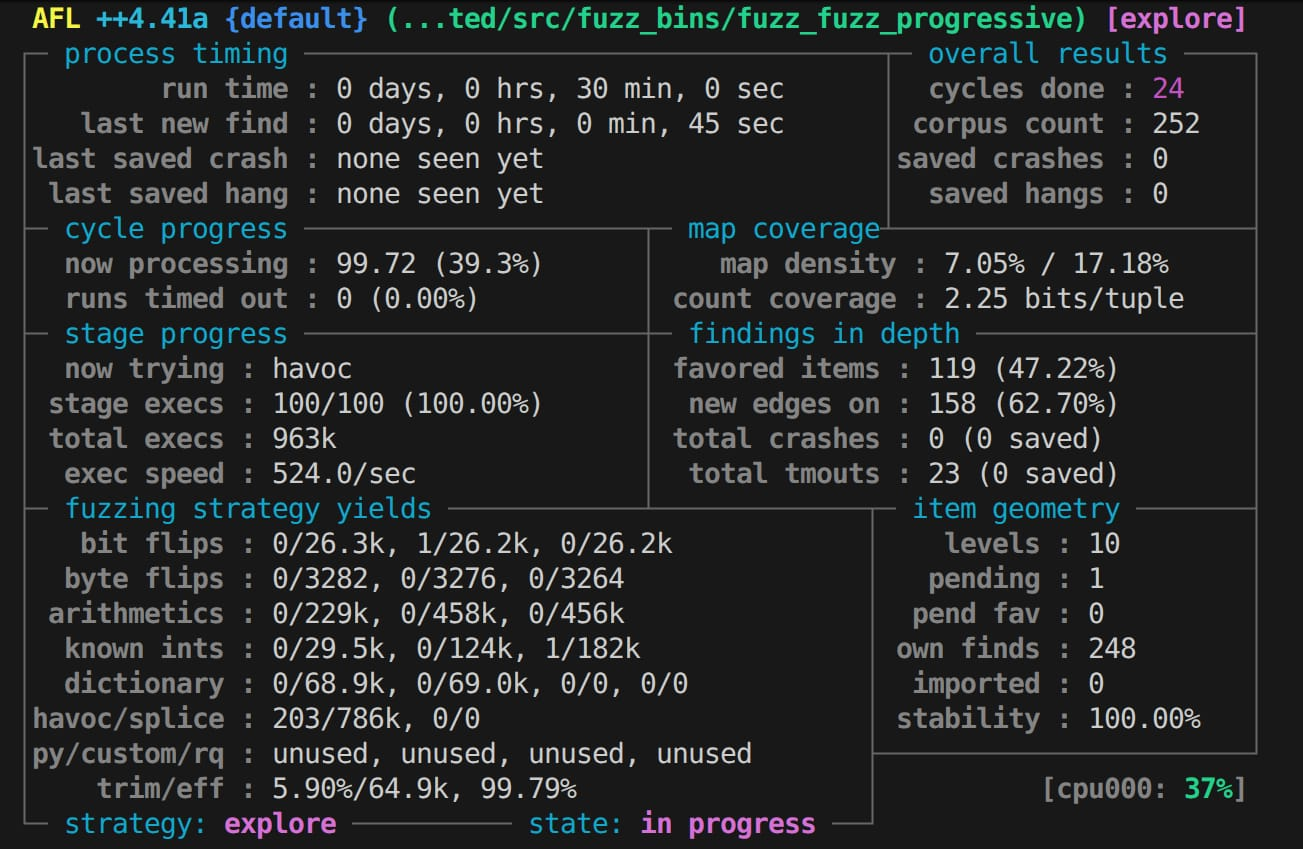
\includegraphics[width=0.5\linewidth]{Figures/statusInstruProg.jpeg}
    \caption{Status screen at end of instrumented run (progressive)}
    \label{fig: statusInstru}
\end{figure}
\begin{figure}
    \centering
    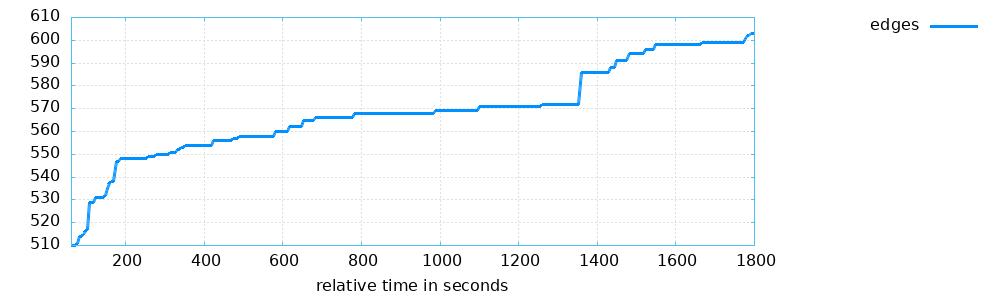
\includegraphics[width=0.5\linewidth]{Figures/edgesInstruProg.png}
    \caption{afl-plot edges graph of the instrumented run (progressive)}
    \label{fig: edgeInstru}
\end{figure}
\begin{figure}
    \centering
    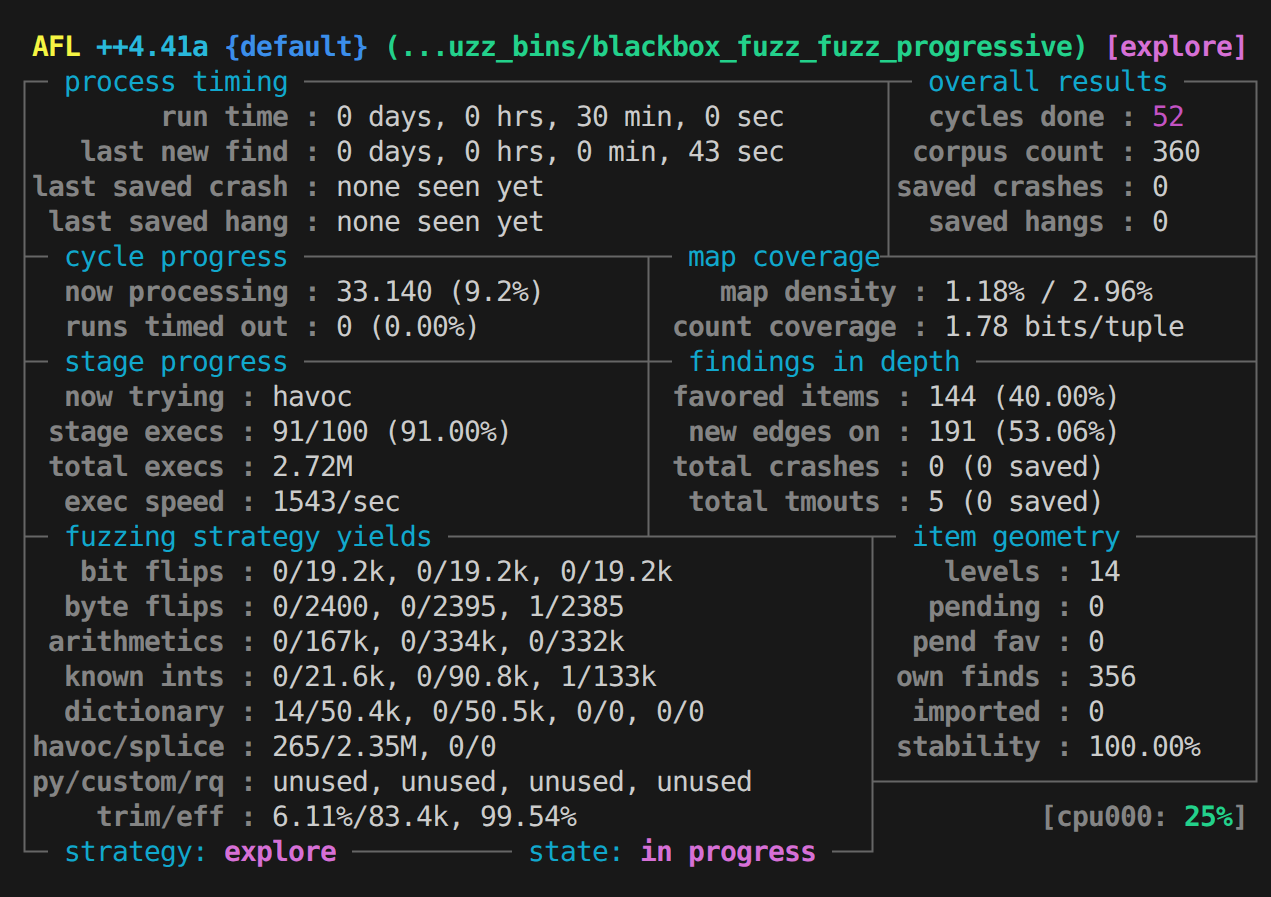
\includegraphics[width=0.5\linewidth]{Figures/image.png}
    \caption{Status screen at end of QEMU run (progressive)}
    \label{fig: 7.1}
\end{figure}
\begin{figure}
    \centering
    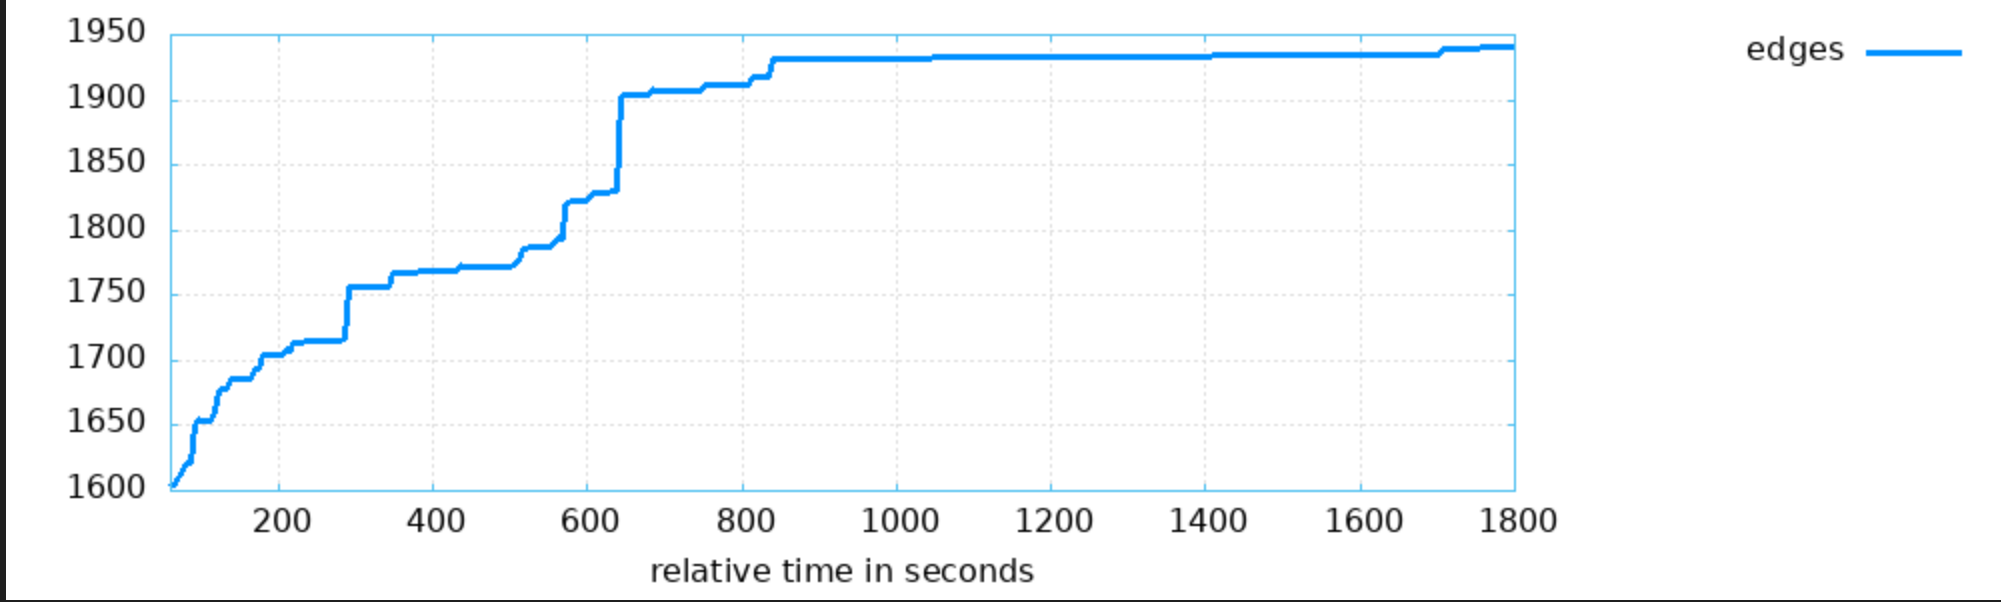
\includegraphics[width=0.5\linewidth]{Figures/graph.png}
    \caption{afl-plot edges graph of the QEMU run (progressive)}
    \label{fig: 7.2}
\end{figure}


%%%%%%%%%%%%%%%%%%%%%%%%%%%%%%%%%%%%%%%%%%%%%%%%%%%%%%%%%%%%%%%%%%%%%%%%%%%%%%%%
\end{document}
%%%%%%%%%%%%%%%%%%%%%%%%%%%%%%%%%%%%%%%%%%%%%%%%%%%%%%%%%%%%%%%%%%%%%%%%%%%%%%%%

%%  LocalWords:  endnotes includegraphics fread ptr nobj noindent
%%  LocalWords:  pdflatex acks